
\documentclass[12pt,letterpaper]{report}
\usepackage[margin=1in]{geometry}
\usepackage{graphicx}
\usepackage{amsmath}
\usepackage[font=small,labelfont=bf]{caption}
\usepackage[justification=centering]{caption}
\newlength \figwidth
\setlength \figwidth {0.75\linewidth}

\begin{document}

\title{E153 Laboratory Assignment \#2}
\author{Courtney Keeler and Stephen Pinto\\
Harvey Mudd College}
\date{September 30, 2013}
\maketitle

\section*{List of Materials}
\begin{itemize}
	\item Tektronix 2212 Oscilloscope
	\item Pomona 4550B (10X probe)
	\item Elenco LCM-1950 Multimeter
	\item Pre-built mystery circuits
\end{itemize}

\section*{Purpose}
The purpose of this lab is to apply the knowledge learned in Lab \#1 about the difference between a BNC cable and a 10X probe, and how to analyze signals captured with both devices.

\section*{Mystery Circuit}
\subsection*{Procedure}
\begin{enumerate}
\item View the output waveform of circuit A using the Tektronix 2212 Oscilloscope and BNC cable
\item Repeat the previous step using the 10X probe
\item Repeat the two previous steps for circuit B
\end{enumerate}

\subsection*{Results}

\begin{figure}
\centering
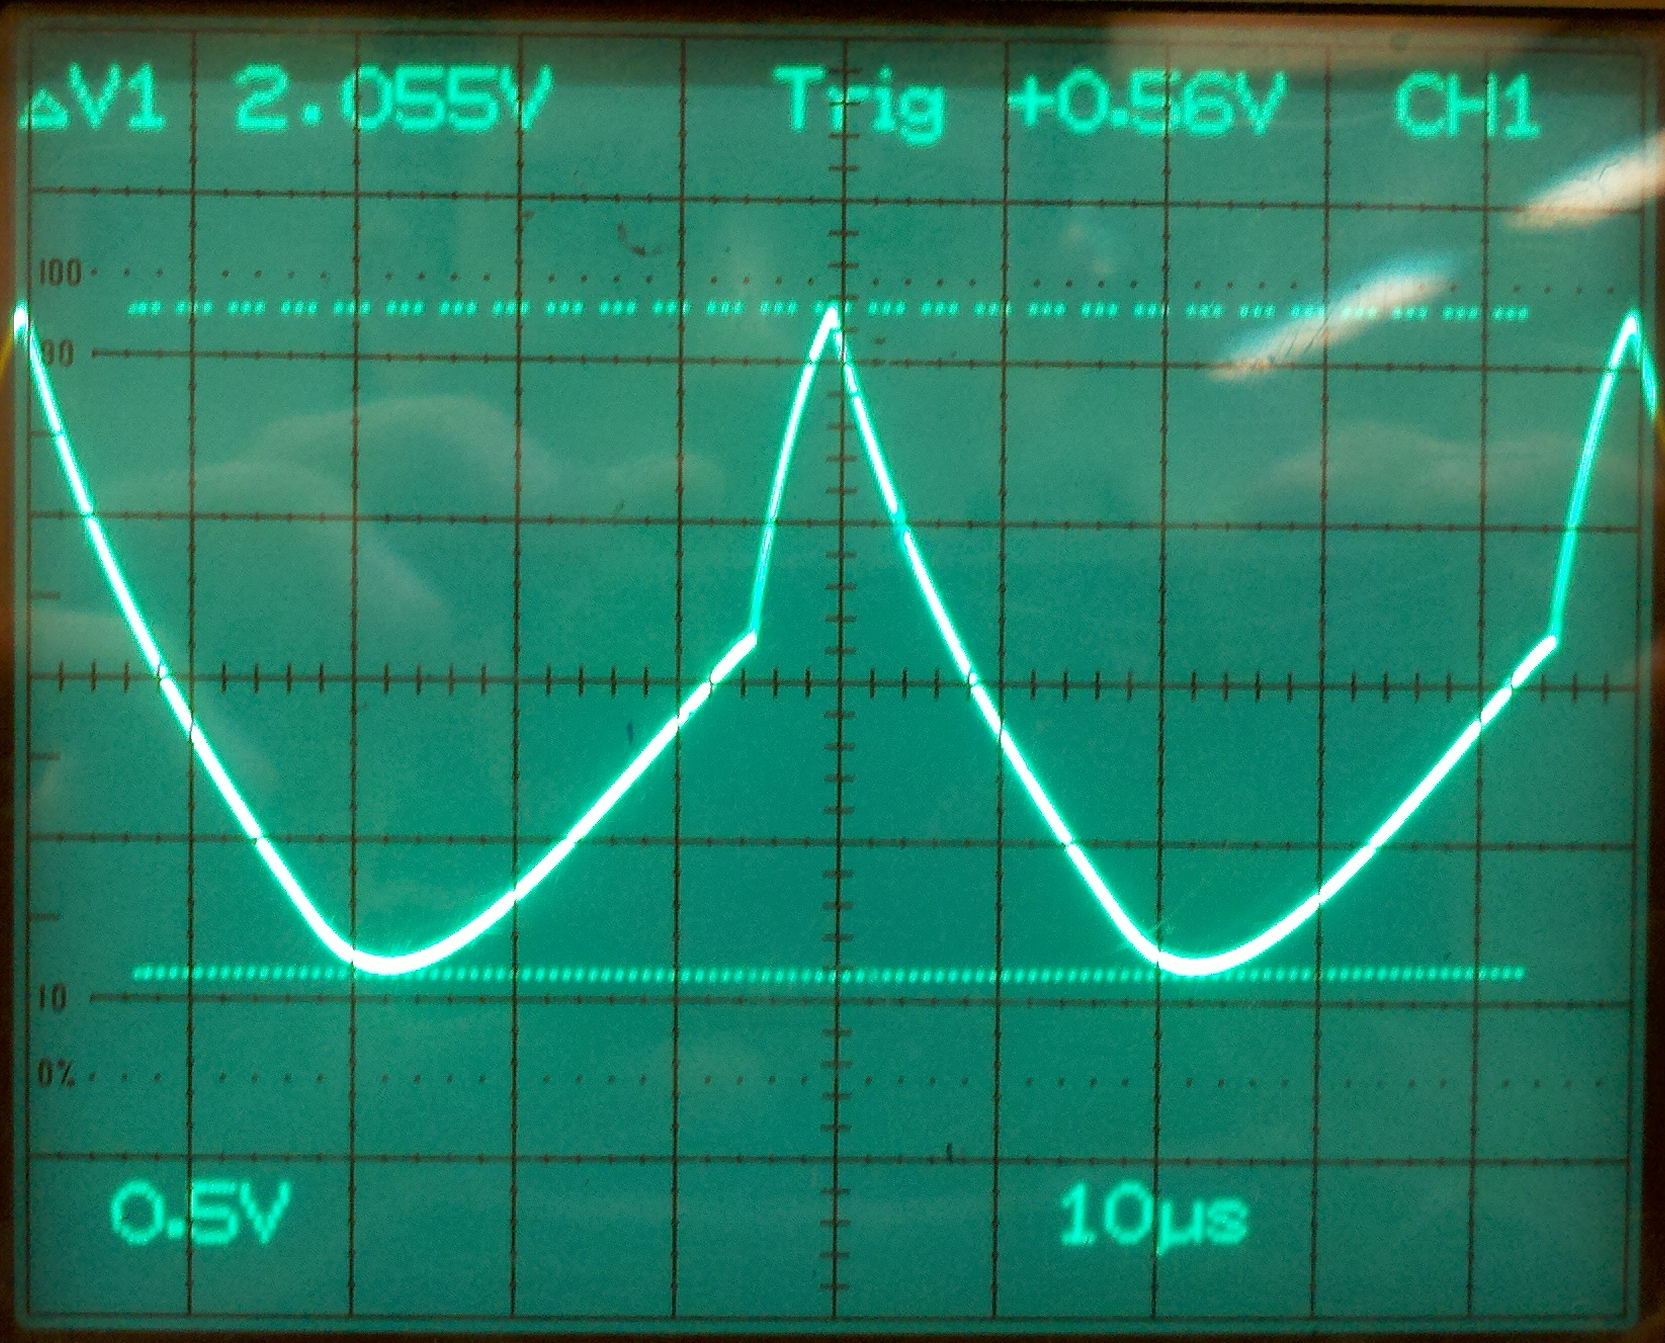
\includegraphics[width=\figwidth, keepaspectratio=true]{lab2/lab2_images/BNC_CircuitA.png}
\caption{Output waveform of circuit A, measured using the BNC cable and oscilloscope.}
\label{fig:bnc_circuit_A}
\end{figure}

\begin{figure}
\centering
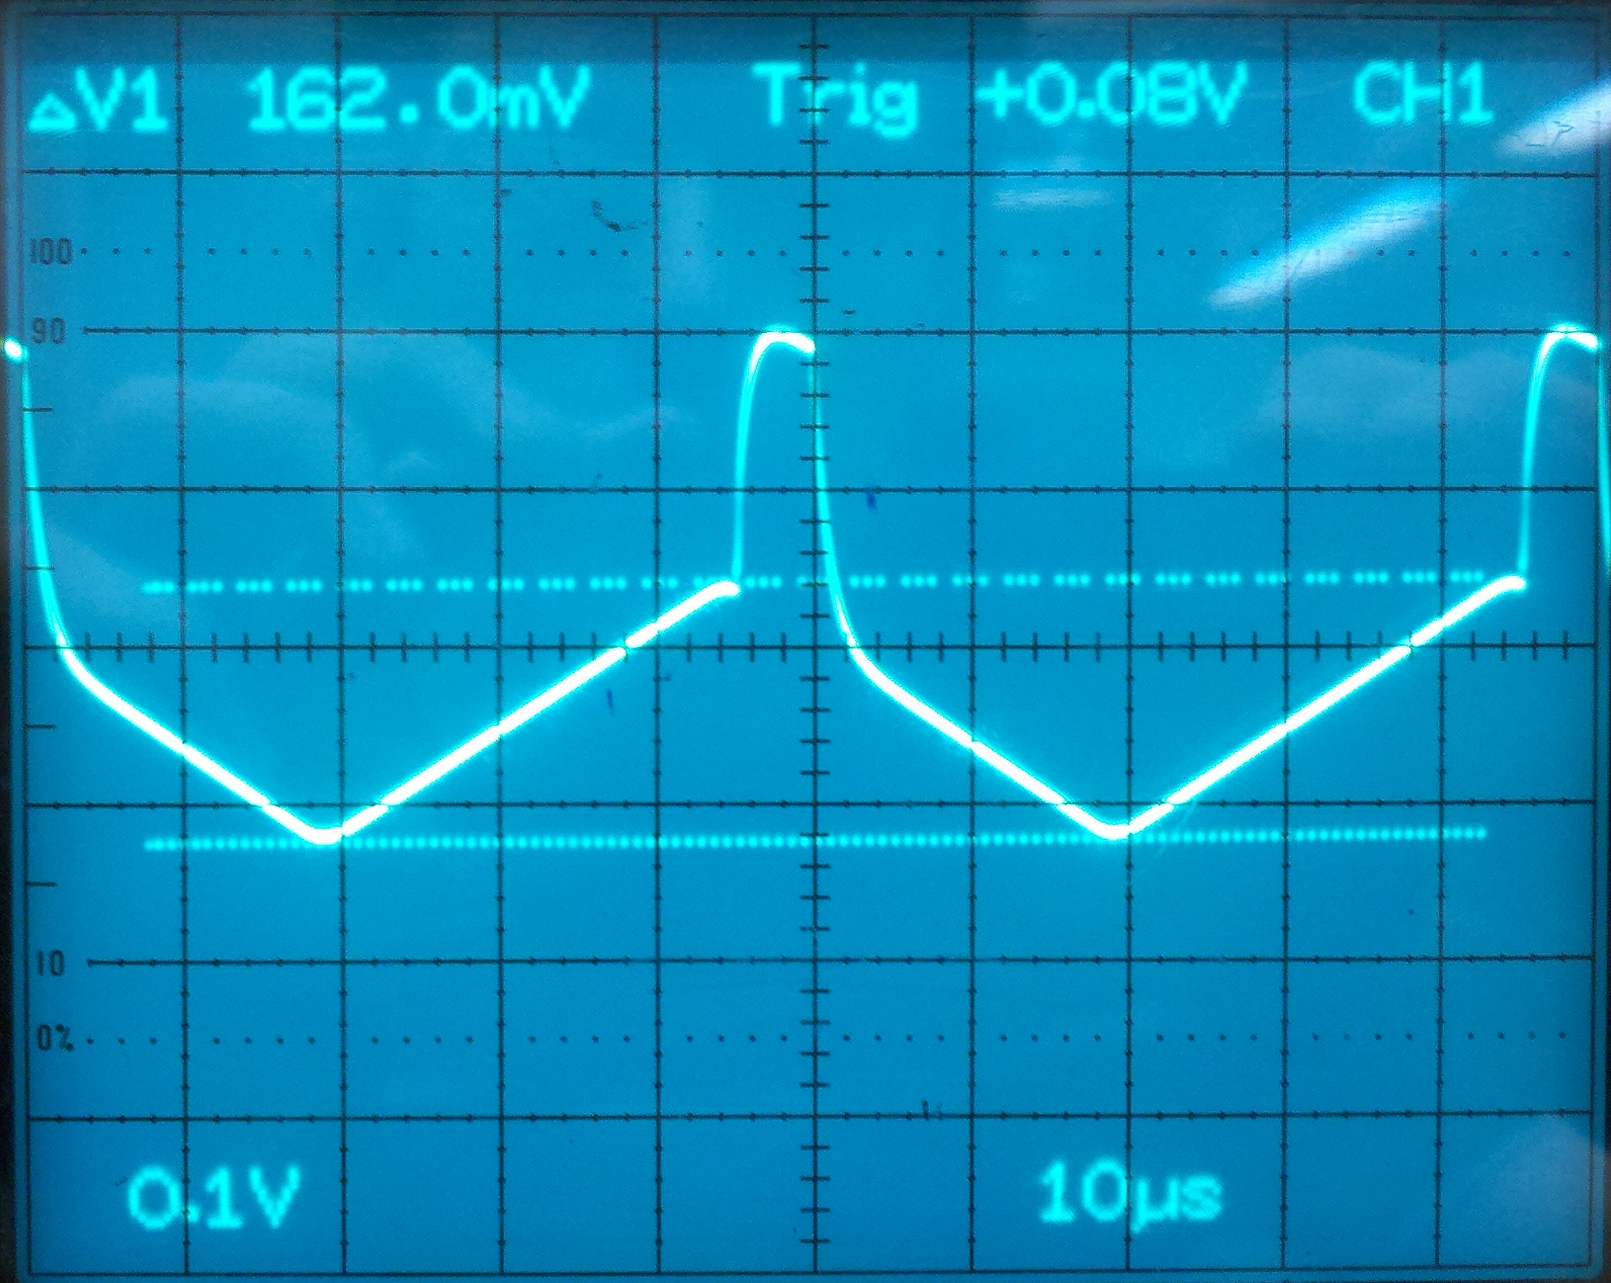
\includegraphics[width=\figwidth, keepaspectratio=true]{lab2/lab2_images/10x_CircuitA_2.png}
\caption{Output waveform of circuit A, measured using the 10X probe and oscilloscope.}
\label{fig:10x_circuit_A}
\end{figure}

\begin{figure}
\centering
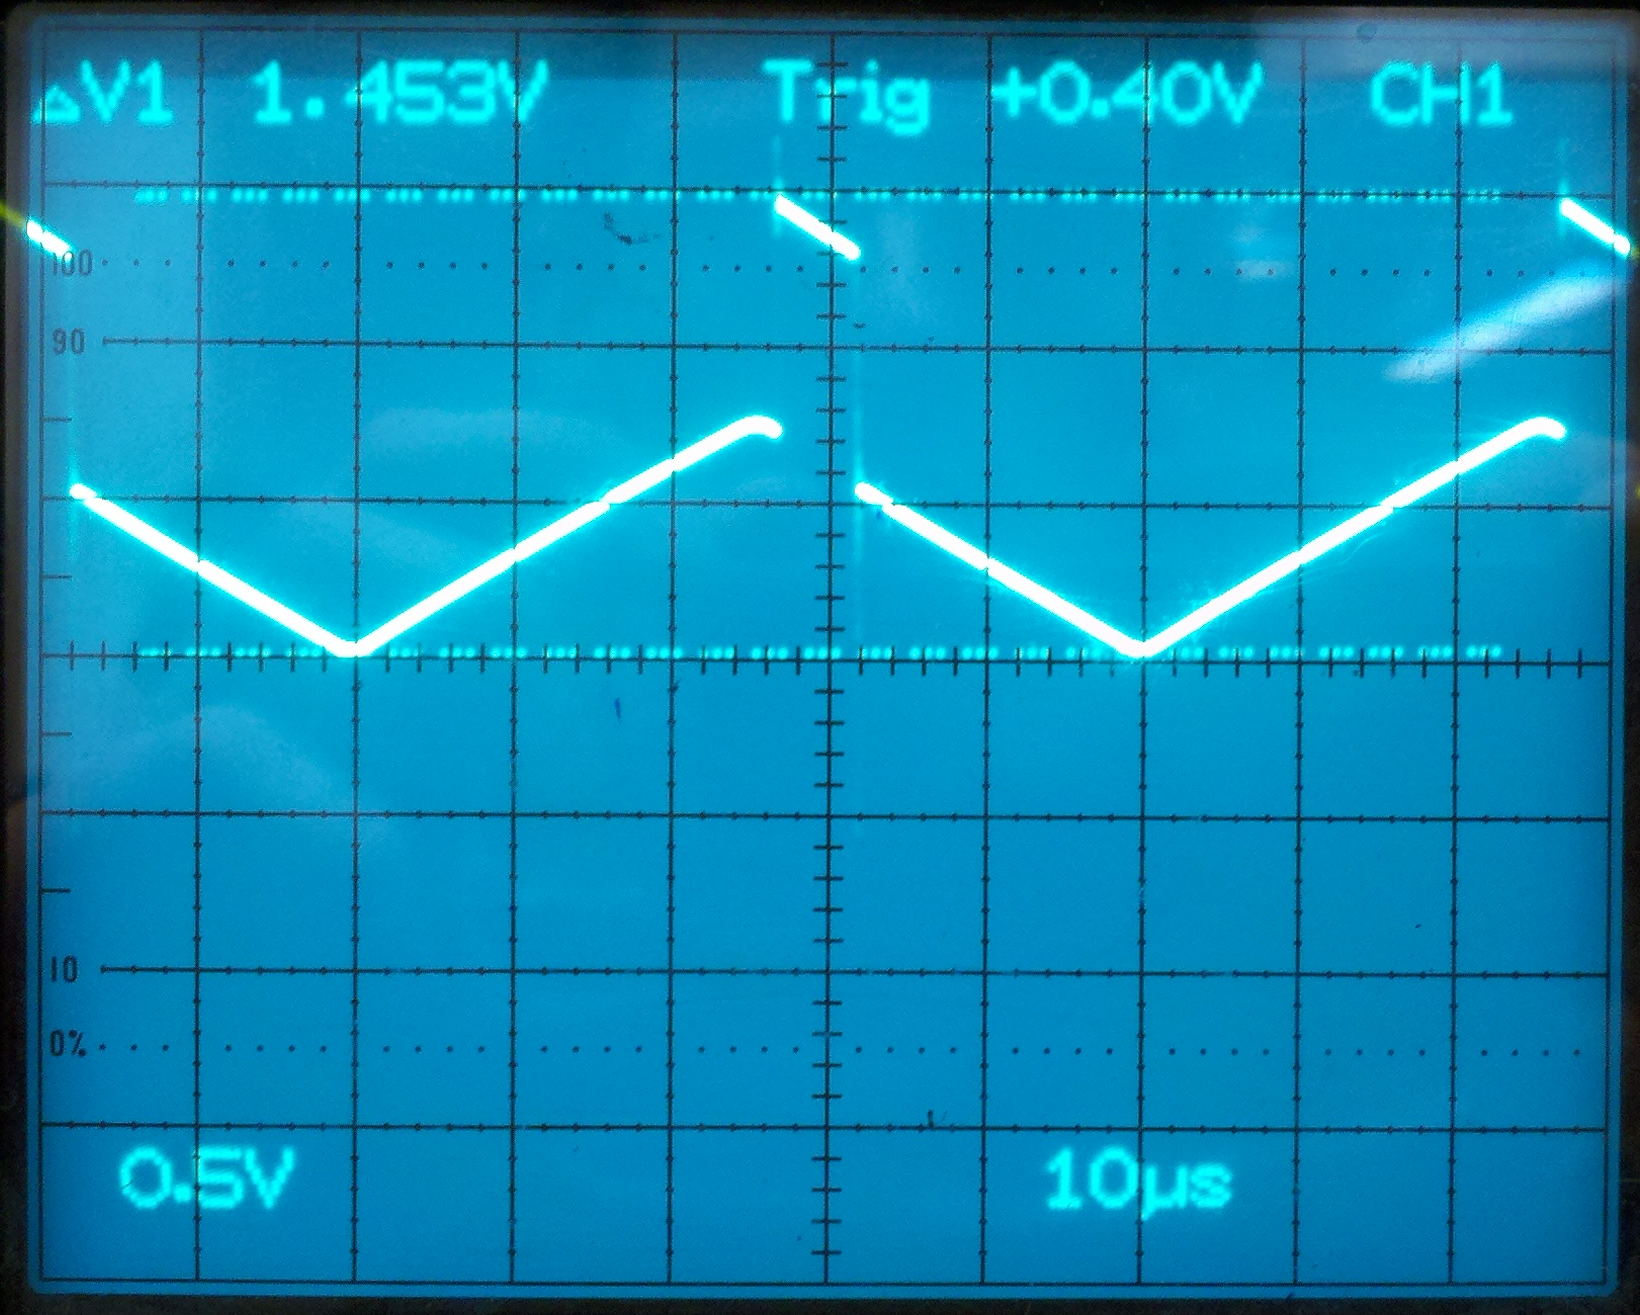
\includegraphics[width=\figwidth, keepaspectratio=true]{lab2/lab2_images/BNC_CircuitB.png}
\caption{Output waveform of circuit B, measured using the BNC cable and oscilloscope.}
\label{fig:bnc_circuit_B}
\end{figure}

\begin{figure}
\centering
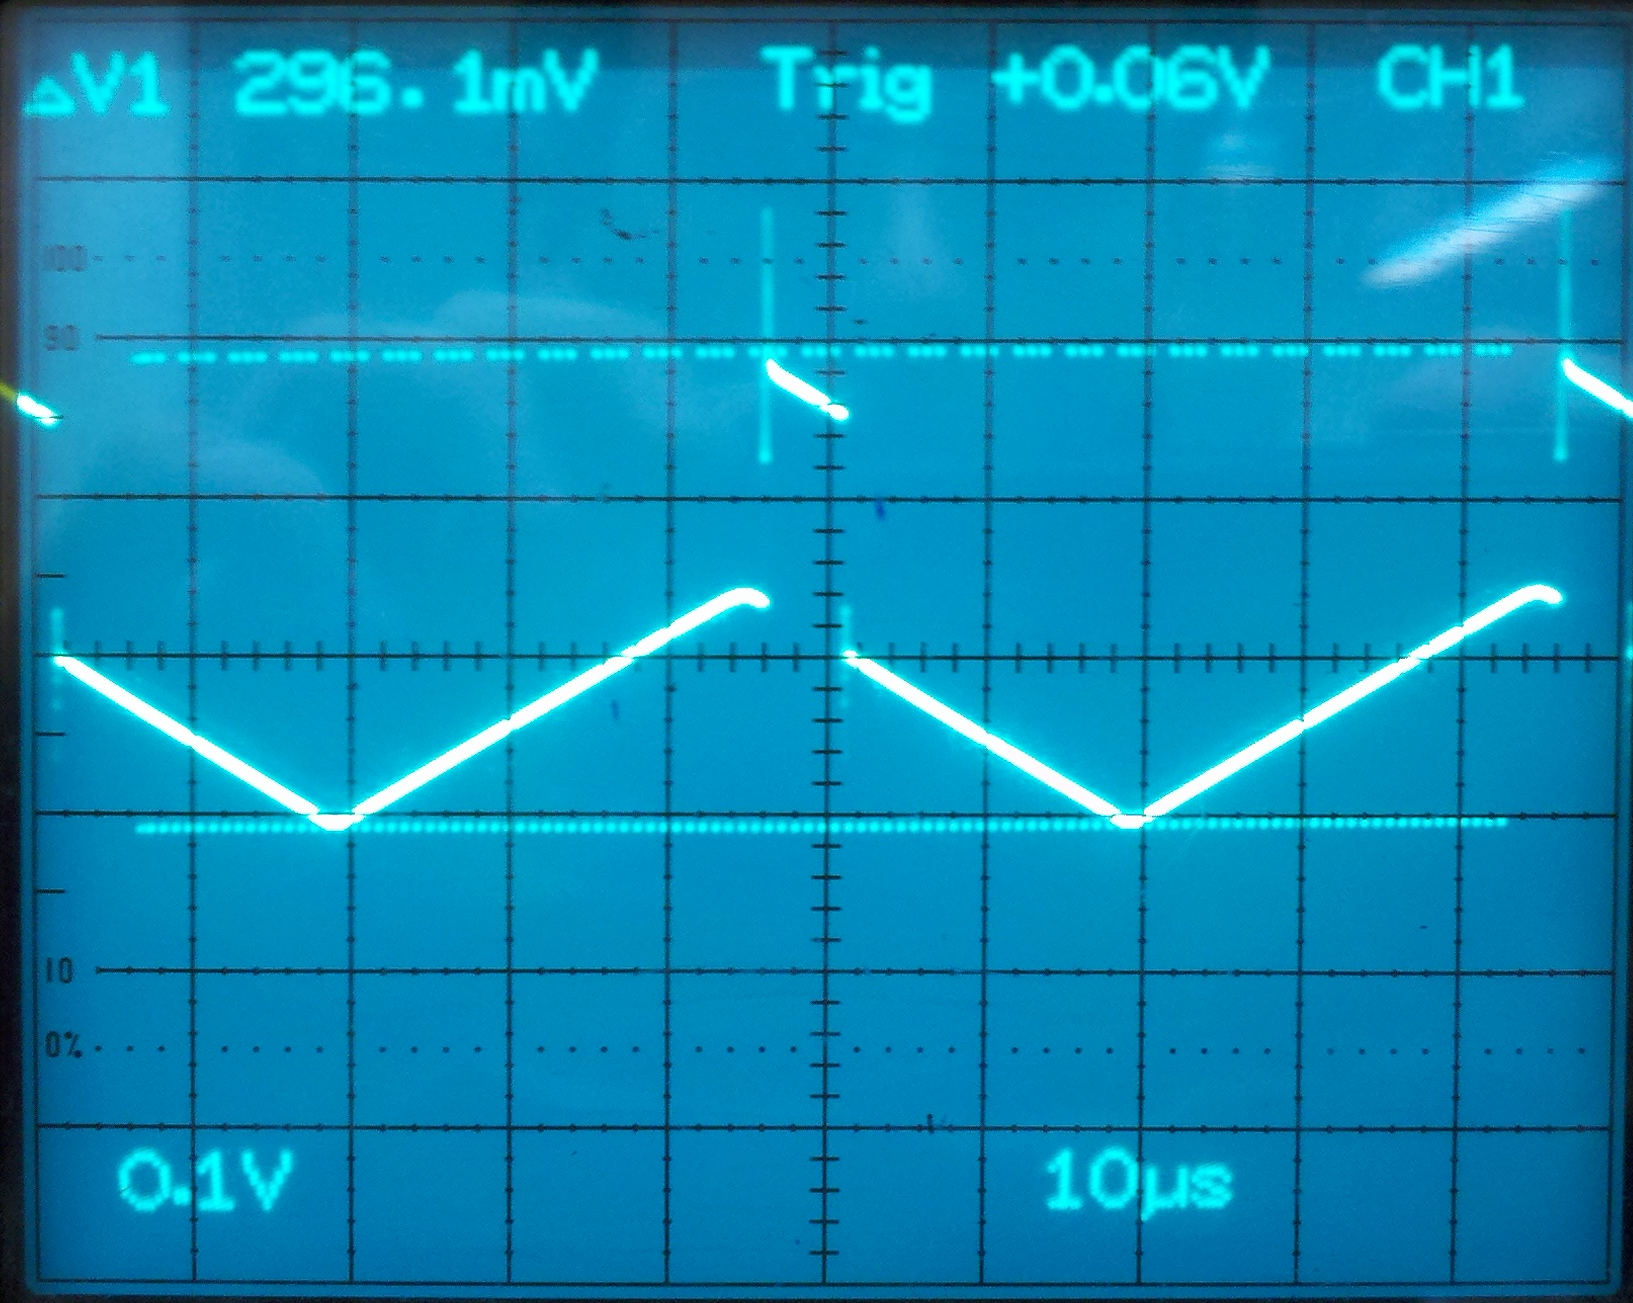
\includegraphics[width=\figwidth, keepaspectratio=true]{lab2/lab2_images/10x_CircuitB.png}
\caption{Output waveform of circuit B, measured using the 10X probe and oscilloscope.}
\label{fig:10x_circuit_B}
\end{figure}

The fundamental frequency of the waveform shown in Figures \ref{fig:bnc_circuit_A} through \ref{fig:10x_circuit_B} is 20.33 kHz. The peak to peak voltage of the triangle wave components for the four waveforms are summarized in Table \ref{table:vpp}.

\begin{table}[ht]
\caption{$\text{V}_{\text{pp}}$ of Triangle Waves} % title of Table
\centering 
    \begin{tabular}{| c | c | c |}
    \hline  
    Circuit & Measuring Device & $\text{V}_{\text{pp}}$ \\
    \hline
    A & BNC & 1.16 V \\
    A & 10X Probe & 162 mV \\
    B & BNC & 1.453 V \\
    B & 10X Probe & 296.1 mV \\
    \hline
    \end{tabular}
    \label{table:vpp}
\end{table}

\end{document}